\documentclass{article}
\usepackage[utf8]{inputenc}
\usepackage[T1]{fontenc}
\usepackage[catalan]{babel}
\usepackage[vmargin=3cm]{geometry}
\usepackage{lastpage}
\usepackage{lipsum}
\usepackage{graphicx}
\usepackage{parskip}
\usepackage{listings, listings-rust}
\usepackage{hyperref}
\usepackage{url}

\hypersetup{
    colorlinks=true,
    linkcolor=black,
    urlcolor=blue,
    citecolor=red,
}

\graphicspath{ {images/} }

\lstnewenvironment{code}[1][]%
{
   \noindent
   \minipage{\linewidth} 
   \vspace{0.5\baselineskip}
   \lstset{language=Rust, style=colouredRust,#1}}
{\endminipage}

\begin{document}
\begin{titlepage}
	\newcommand{\HRule}{\rule{\linewidth}{0.4mm}} % Defines a new command for horizontal lines, change thickness here
	
	\center

    \vspace*{25px}
    % == Headings ==
	
	\textsc{\LARGE Universitat Autònoma de Barcelona}\\[1.5cm]
	
	\textsc{\Large Treball de Fi de Grau}\\[0.5cm]
	
	\textsc{\Large Informe inicial}\\[0.5cm]
	
	\HRule\\[0.4cm]
	
	{\LARGE\bfseries Disseny i implementació d'un llenguatge de programació amb LLVM}\\[0.4cm]
	
	\HRule\\[1.5cm]
	
	% == Author ==
	
	\begin{minipage}{0.5\textwidth}
		\begin{flushleft}
			\large
			\textit{Autor}\\
			\textsc{Josep Maria Domingo Catafal}
		\end{flushleft}
	\end{minipage}
	~
	\begin{minipage}{0.4\textwidth}
		\begin{flushright}
			\large
			\textit{Tutor}\\
			\textsc{Javier Sánchez Pujadas}
		\end{flushright}
	\end{minipage}
	
	% == Date == 

	\vfill\vfill\vfill % Position the date 3/4 down the remaining page
	
	{\large\today} % Date, change the \today to a set date if you want to be precise

	\vfill % Push the date up 1/4 Of the remaining page
\end{titlepage}

% --------------------------------------
% Table of contents
% --------------------------------------
\tableofcontents
\newpage

% --------------------------------------
% Body
% --------------------------------------
\section{Introducció i el problema a resoldre}
Històricament, hi ha hagut sempre un dilema entre la rapidesa d'execució, i la
rapidesa de desenvolupament.

Alguns llenguatges són fàcils de programar: permeten al programador
despreocupar-se de conceptes de baix nivell com ara la gestió de la memòria,
i creen abstraccions que agilitzen el desenvolupament. El problema és que
aquestes abstraccions, limiten l'eficiència del llenguatge, i creen programes
més lents. Un altre motiu que permet agilitzar el desenvolupament és el tipat
dinàmic, ja que permet despreocupar-se de quin tipus s'ha de fer servir. Però
això també té els seus inconvenients, donat que és molt probable que et trobis amb
errors en temps d'execució. Aquests llenguatges també acostumen a ser interpretats
per tal d'estalviar al programador l'espera de compilar el programa, però té
un impacte en el rendiment d'execució del programa si ho comparem amb llenguatges
compilats. Python seria un dels majors representants d'aquest grup de llenguatges.

En l'altra cara de la moneda i tenim llenguatges com C, els quals no tenen gairebé
cap abstracció i el programador ha de ser conscient del que fa amb la memòria en
cada línia de codi que escriu. Són llenguatges que aporten un molt bon rendiment,
però alenteixen molt el desenvolupament, ja que el programador ha de tenir en
compte molts conceptes de baix nivell.
Un problema addicional és que al gestionar la memòria de forma manual, s'obre
la porta a una gran quantitat d'errors en temps d'execució en la forma de
memory leaks. Actualment, hi ha llenguatges com Rust que soluciones aquestes
qüestions de gestió de memòria sense perdre rendiment, però el desenvolupament
continua sent lent i el temps de compilació llarg. Aquests llenguatges, també
acostumen a ser fortament tipats, cosa que redueix els errors en temps
d'execució, però alenteix el desenvolupament.


\section{Objectiu}

Podem veure que disposem de dos paradigmes ben oposats: un busca el rendiment a
canvi d'un desenvolupament lent, mentre l'altre prefereix agilitzar el
desenvolupament, però alentir l'execució. L'objectiu d'aquest treball,
és crear un llenguatge de programació que se situï al mig d'aquests dos
paradigmes, fent sacrificis per ambdues bandes.

Sacrificis en l'agilitat de desenvolupament:
\begin{itemize}
    \item \textbf{Compilat}: Serà un llenguatge compilat, per tal d'obtenir un
        bon rendiment i evitar al màxim els erros en temps d'execució.
    \item \textbf{Fortament tipat}: Per evitar al màxim l'aparició d'errors en
        temps d'execució, i també perquè ajuda a documentar el codi, facilitant
        la seva lectura.
    \item \textbf{Immutabilitat}: S'intentarà forçar la immutabilitat sempre que
        sigui possible, per així evitar els efectes secundaris, i facilitar la depuració
        del codi
\end{itemize}

Sacrificis en el rendiment d'execució
\begin{itemize}
    \item \textbf{Gestió de memòria automàtica}: L'usuari no s'haurà de preocupar
        d'eliminar la memòria de forma manual. Hi haurà un Garbage Collector,
        cosa que penalitza en el rendiment, però redueix memory leaks i agilitza
        el desenvolupament.
\end{itemize}

\section{Definició del llenguatge}

Per importar llibreries externes s'utilitzen imports

\begin{code}
import math
\end{code}

Podem definir constants globals, però no variables. Amb això es busca evitar
comportaments estranys del programa i bugs difícils de trobar, ja que les
variables globals poden ser modificada des de qualsevol lloc i costa trobar
qui és que l'està canviant.

\begin{code}
const MAX_SPEED = 120;
\end{code}

El punt d'inici del programa és a la funció main.

\begin{code}
fn main() {
    // Les instruccions acaben sempre amb un punt i coma
    println("Hello World!");
}
\end{code}

Per declarar una funció es fa amb la paraula reservada fn, seguit del nom de la
funció i els paràmetres entre parèntesis, i finalment el tipus del valor de retorn.
Quan l'última expressió no acaba en punt i coma, el resultat serà el que retornarà
la funció. És l'únic cas en què es permet no posar punt i coma.

\begin{code}
fn radius(circumference: i32) i32 {
    circumference / (2 * math.PI)
}
\end{code}

\subsection{Definició de tipus}

Si volem definir tipus genèrics, podem definir interfícies:

\begin{code}
interface Person {
    fn change_name(name: string) string;
}
\end{code}

Això ens permet tenir diferents implementacions, amb comportaments diferents.

Per crear tipus propis, es fan servir structs. Permeten definir camps de diferents
tipus i definir mètodes que modifiquen l'estat de l'objecte.

Els camps i els mètodes, per defecte són privats, però es poden fer públics.
En el cas de les funcions amb la paraula reservada "pub". En el cas dels camps,
afegim entre claus (\{\}), les paraules get o set, depenent de si volem que sigui pública
per escriptura, lectura o per les dues coses.

Per implementar una interfície, afegim dos punts i el nom de la interfície just
després del nom del struct.

\begin{code}
struct User : Person {
    age: i32 { get, set };
    name: string { get };
    id: i32;

    fn change_name(name: string) {
        self.name = name;
    }
}
\end{code}

Amb l'struct anterior, podríem per exemple fer el següent:

\begin{code}
let user = User { age: 24, name: "John Doe" };
user.age = 25;
println(user.name);
\end{code}

Però no podríem modificar el camp \textit{name}.

No és obligatori definir constructor, però si es vol, l'estàndard és crear una
funció estàtica que es digui \textit{new}.

\begin{code}
// constructor
pub static fn new(age: i32, name: string) self {
    self {
        age,
        name,
    }
}
\end{code}

Per cridar les funcions estàtiques es fa de la següent manera:

\begin{code}
// static: struct_name::static_fn()
let user = User::new(24, "John Doe");
// non-static: object.fn()
user.change_name("Jane Doe");
\end{code}

Podem definir mètodes fora de la definició del struct. Un cas on seria útil,
per exemple, seria quan treballem amb una entitat amb moltes funcions i volem
dividir-ho en múltiples fitxers.

\begin{code}
struct User {
    name: string;
}

pub fn (User) get_name() string {
    self.name
}
\end{code}

Quan un mètode muta l'estat d'un objecte, aquesta funció ho ha d'indicar de forma
explícita. Amb això es busca facilitar la vida al programador a l'hora de programar,
llegir el codi o depurar, ja que només llegint la crida o la definició, sap que
la funció té efectes secundaris.

Per tal d'indicar aquesta mutació, el programador, ha d'afegir la paraula "mut",
a la definició de la funció, i cada cop que la crida, s'ha d'afegir un signe
d'exclamació al final de l'identificador (ex: {\ttfamily function!(a, b)}).

El mateix passa amb les variables. Per defecte són immutables. Si es vol mutar
una variable, s'ha d'afegir la paraula "mut".

\begin{code}
struct User {
    name: string;
    pub mut fn set_name(self, name: string) string {
        self.name = name;
    }
}

fn modify_struct() {
    let mut user = User::new();
    user.set_name!("new name");
}
\end{code}

\subsection{Bucles}

Per tal d'executar repetidament instruccions es fan servir bucles. N'hi ha de
diferents tipus. El més bàsic és el while:

\begin{code}
let mut a = 0;
let mut i = 0;
while i < 10 {
    a += i;
    i += 1;
}
\end{code}

Un altra opció, és el bucle for:

\begin{code}
let mut a = 0;
// No need for "mut" when declaring variables on for loop declarations, it's implied
for let i = 0; i < 10; i += 1 {
    a += i;
}
\end{code}

Per iterar arrays, tenim el bucle for in, que recorre l'array element per element.

\begin{code}
let mut a = 0;
for number in numbers {

}
\end{code}


Podem fer break d'un bucle en concret posant una etiqueta:

\begin{code}
// Break outer loop from inner loop
outer: for number in numbers {
    for number in numbers {
        if number % 2 == 0 {
            break outer;
        }
    }
}
\end{code}

O fer un break normal:

\begin{code}
for number in numbers {
    if number % 2 == 0 {
        break;
    }
}
\end{code}

\subsection{Programació Funcional}

Per tal de simplificar algunes operacions que es realitzen amb freqüència, hi
haurà algunes funcions com ara map, reduce, fold, etc. que ens permetran
escriure aquestes operacions amb moltes menys línies. Per tal de poder fer servir
aquestes funcions, es farà ús de "closures" o clausures.

\begin{code}
fn functional_style(numbers: [i32]) {
    // Functional style with closures
    let numbers_plus_one = numbers.map(|x| -> x + 1);

    let sum = numbers.reduce(|sum, number| -> {
        if number % 2 == 0 {
            sum + number
        }
    });

    if number.any(|x| -> x > 5) {
        print("There's at least one number greater than 5");
    }

    if number.all(|x| -> x > 5) {
        print("All numbers are greater than 5");
    }
}
\end{code}

Les clausures ens permeten tenir funcions de primer ordre, el que vol dir que
les podem tractar com a qualsevol expressió, assignant-les a una variable, per 
exemple, o sent retornades per una altra funció.

\begin{code}
fn two_plus_two() {
    let sum = |a: int, b: int| int -> {
        a + b
    };
    print(sum(2, 2)); // Output: 4
}
\end{code}

Un altre concepte inspirat en llenguatges funcionals, és l'operador pipe (|>). 
Ens permet millorar la lectura de casos tipus el següent:

\begin{code}
validate_age(get_age(parse_data(person)))
\end{code}

Que passaria a ser així:

\begin{code}
let is_valid = 
    person
    |> parse_data
    |> get_age
    |> validate_age;
\end{code}

El que fa el pipe, és passar l'expressió de l'esquerra, com a paràmetre de la
funció que hi ha a la dreta.

\subsection{Gestió d'errors}

Les funcions poden retornar el que se'n diu un Result. Un Result, és un enum
que té dos valors possibles: {\ttfamily Ok(T) i Err(E)}, on T és l'element que retorna la
funció, i E és l'error que retorna la funció.

En indicar el tipus de retorn com a Result, hem d'indicar el tipus del valor que
retorna la funció, i el tipus de l'error: {\ttfamily Result<TipusOk, TipusErr> }

\begin{code}
fn divide(a i32, b i32) Result<i32, string> {
    if b == 0 {
        return Err("Divide by zero");
    }
    return Ok(a / b)
}
\end{code}

Quan cridem a la funció, hem de comprovar que no ens hagi retornat cap error:

\begin{code}
fn call_divide() -> Result<i32, string> {
    let result = match divide(5, 0) {
        Ok(num) => num,
        Err(err) => return Err(err),
    }

    print("The result is: ", result);
    Ok(result)
}
\end{code}

Com que pot ser una mica empipador haver de comprovar l'error en cada crida, hi
ha l'operador "?" que ens permet retornar immediatament en cas que el resultat
sigui un error:

\begin{code}
fn call_divide() -> Result<i32, string> {
    let result = divide(5, 0)?;
    print("The result is: ", result);
    Ok(result)
}
\end{code}

D'aquesta manera, com que la funció divide ens retorna un error, call\_divide,
retorna immediatament l'error i ja no s'executa el print. En cas que divide hagués
retornat un Ok, l'execució hagués continuat. Cal destacar que la funció que 
fa servir l'operador "?", també ha de retornar un Result, ja que implica que pot
retornar un error.

\subsection{Referències}

Si a un tipus l'hi afegim un {\ttfamily \&} a davant, passarà a ser una referència. Les
referències en permeten apuntar directament a una posició de memòria, i passar
aquest apuntador, sense la necessitat de copiar l'objecte. Per defecte les
referències, igual que les variables, són immutables, però es poden mutar, si
afegim la paraula mut. En cas que la referència sigui mutable, es modificarà
la posició de memòria a on apunta, per tant, totes les referències que llegeixin
d'aquesta posició de memòria veuran el canvi. És a dir, venen a ser apuntadors
ensucrats, similar a C++.

\begin{code}
// References are immutable by default but we can make them mutable
fn references(numbers: &[i32], other_numbers: &mut [i32]) {
    for number in numbers {
        print(number);
    }

    for number in other_numbers {
        *number += 1; // This will modify the original vector
    }
}
\end{code}

\section{Passos a seguir}

Abans de començar a fer qualsevol cosa, hem d'escollir la tecnologia amb la qual
volem implementar el compilador. Per aquest projecte, s'ha escollit a Rust com
llenguatge de programació i a LLVM \cite{llvm_website} com a toolchain per a la generació de codi
del back-end. LLVM ens permetrà generar assemblador per pràcticament qualsevol
arquitectura que existeixi avui en dia, sense haver de fer cap esforç addicional.
Només ens haurem d'encarregar de generar la IR de LLVM, i aquest s'encarregarà de
generar l'assemblador a partir de l'IR. L'API de LLVM està només per C/C++, per
tant, també farem servir una llibreria que es diu Inkwell \cite{inkwell}, que ens ofereix una
API per a Rust, interactuant amb l'API de C.

Un cop escollides les tecnologies el següent pas és crear un entorn i una
estructura de projecte base, on hi podem anar afegint totes les funcionalitats
addicionals.

Per tal d'implementar les funcionalitats definides, seguirem un procés similar
amb totes. Haurem de fer tres coses:

\begin{enumerate}
    \item \textbf{Lexer}: El lexer s'encarrega de llegir el nostre codi, i
        convertir-lo a un seguit de tokens. Un token és un conjunt de caràcter
        en el codi font que té algun significat en el llenguatge, com ara una paraula
        clau del llenguatge (if, for, ...), o l'identificador d'una variable.
        Per cada funcionalitat, haurem d'adaptar el Lexer perquè ens reconegui
        aquests nous tokens que s'introdueixin al llenguatge.
    \item \textbf{Parser}: El parser recorre la seqüència de tokens que ens
        retorna el lexer i l'hi busca el significat. El resultat del parser és
        un arbre sintàctic, que ens indicarà com s'han d'executar les instruccions.
        Per cada nova funcionalitat, haurem de modificar el parser perquè pugui
        interpretar els nous constructes.
    \item \textbf{Generació de codi}:
\end{enumerate}


\section{Metodologia i planificació}
Per tal d'organitzar el desenvolupament del projecte s'ha optat per una metodologia
basada en sprints, on cada sprint té una duració d'una setmana. Donat que és un
projecte gran, s'ha dividit en un conjunt d'èpiques, que representen un conjunt
de funcionalitats. Cada una d'aquestes èpiques, conte un seguit de subtasques, i
completar cada una d'aquestes èpiques requereix d'uns quants sprints. Les èpiques
que s'han definit són les següents:

\begin{enumerate}
    \item \textbf{Implementació mínima de l'especificació}\\
        Implementar tota la funcionalitat bàsica per poder fer programes senzills.
        Inclou operacions aritmètiques, funcions, control de flux bàsic (if
        statements i bucles while) i declaració de variables.

    \item \textbf{Declaració de tipus} \\
        Implementar la funcionalitat necessària per definir tipus de dades
        propis (structs, interficies i type aliases).

    \item \textbf{Collections}\\
        Implementació d'arrays estàtics, arrays dinàmics i tuples.

    \item \textbf{Mecanisme de gestió d'errors}\\
        Implementar un mecanisme per tal de gestionar errors en temps d'execució.

    \item \textbf{Syntactic sugar}\\
        Implementació de "Syntactic sugar", per tal de simplificar operacions
        que s'utilitzen freqüentment. Inclou bucles for in, match (similar a un
        switch), list comprehension, etc.

    \item \textbf{Suport per programació d'estil funcional}\\
        Afegir suport per programació d'estil funcional, integrant funcions com
        ara map, reduce, fold, etc.
\end{enumerate}

Per tal de gestionar totes aquestes èpiques, les seves subtasques i els sprints,
es farà servir Jira, un programa de gestió de projectes que ho facilita molt.

\begin{figure}
    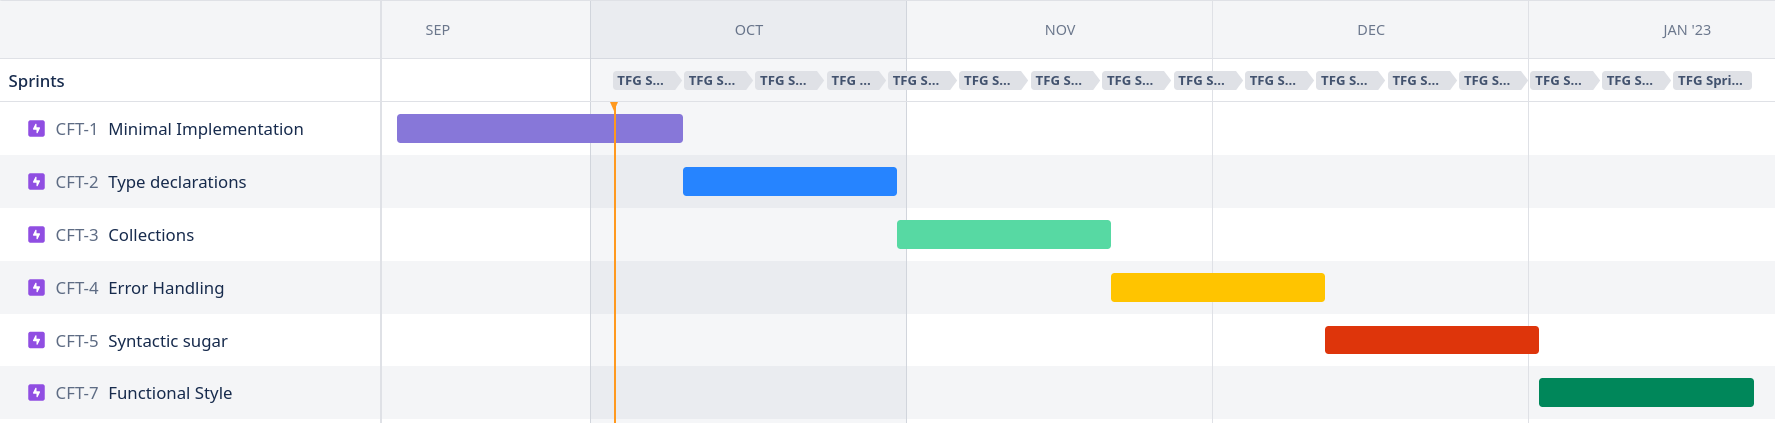
\includegraphics[width=\linewidth]{roadmap}
    \caption{Roadmap on es mostren les diferents èpiques i l'espai de temps on s'han de desenvolupar}
\end{figure}

Cada una d'aquestes funcionalitats, generalment, es divideixen en tres 
subtasques principals: implementar el lexer, implementar el parser i 
implementar la generació de codi.

\section{Inspiració}
La gran majoria de funcionalitats descrites en l'apartat anterior han siguit 
inspirades d'altres llenguatges ja existents. La sintaxi és similar a la de Rust,
però agafant conceptes d'altres llenguatges i paradigmes. Per exemple:

\begin{enumerate}
    \item \textbf{List comprehension}: Python
    \item \textbf{Iteradors (map, reduce, ...)}: Llenguatges funcionals, Javascript, Rust, C\#...
    \item \textbf{Result i Option}: Rust, Scala, Swift
    \item \textbf{Immutabilitat}: Llenguatges funcionals, Rust, Swift
    \item \textbf{Structs}: C, Go, Rust
    \item \textbf{Pipes}: Elixir, F\#
    \item \textbf{Referències}: C++, Rust, Go
    \item \textbf{Sintaxi get, set}: C\#
    \item \textbf{Expression-oriented}: Scala, Rust, Kotlin
\end{enumerate}

\begin{thebibliography}{9}
\bibitem{llvm_website} 
The LLVM Compiler Infrastructure, \url{https://llvm.org}

\bibitem{inkwell} Inkwell, \url{https://github.com/TheDan64/inkwell}

\bibitem{llvm_kaleidoscope} LLVM Kaleidoscope Tutorial: Implementing a Language with LLVM,\\ \url{https://llvm.org/docs/tutorial}

\bibitem{crafting-interpreters}Crafting Interpreters, Bob Nystrom, \url{http://www.craftinginterpreters.com}

\end{thebibliography}
\end{document}
